\newcommand{\jahr}{2018}
\documentclass[a4paper]{article}

\usepackage[T1]{fontenc}
\usepackage[utf8]{inputenc}
\usepackage{graphicx}
\usepackage{xcolor}
\usepackage{fancyhdr}

\graphicspath{{../../../materials/Vorlagen/}{images/}}
\lhead{Rechenschaftsbericht \jahr}
\rhead{\includegraphics[height=1em]{de-RSE-logo-text-colour}}
\pagestyle{fancy}

\usepackage{soul}
\usepackage{longtable}

\usepackage[breaklinks=true]{hyperref}
\def\UrlBreaks{\do\/\do-\do\ }

\usepackage{graphicx}

\renewcommand{\figurename}{Abbildung}



\begin{document}
\thispagestyle{empty}

\begin{centering}
\includegraphics[height=3em]{de-RSE-logo-text-colour}\\
\vspace{3em}
\textbf{
 \Large Rechenschaftsbericht des Vorstands\\*[.5em]
 \normalsize Geschäftsjahr: \jahr}\\*[3em]
\end{centering}

% https://www.vereinswelt.de/rechenschaftsbericht

%Rechenschaftsbericht (wann wurde was von wem gemacht, vor allem ab Gruendung 2018)
%an wen: bestehende, aber vor allem: potentiell neue Mitglieder und Sponsoren
%Dank an Sponsoren, inklusive der der Konferenz (haben ja sonst noch keine)

Dieser Rechenschaftsbericht über die Vereinstätigkeiten wurde auf der Jahreshauptversammlung am 6. Juni in Potsdam vorgestellt.
Der Finanzbericht liegt separat vor.

\section{Mitglieder und Mitgliedsbeiträge}

Der Verein hat zum Ende des Geschäftsjahres 20 Mitglieder.
Alle diese Mitglieder traten bei der Gründungsversammlung am 26. November 2018 ein.
Entsprechend des Beschlusses der Gründungsversammlung wurde für das Jahr 2018 kein Mitgliedsbeitrag erhoben.
Der Beitritt neuer Mitglieder wurde vom Vorstand nicht aktiv beworben, da bis zum Ende des Geschäftsjahres organisatorische und rechtliche Rahmenbedingungen (Konto, Eintragung ins Vereinsregister) noch nicht gegeben waren.

\section{Vorstand}

Dieser Rechenschaftsbericht wird vom Vorstand des Geschäftsjahres 2018 vorgelegt, welcher sich aus folgenden Personen zusammensetzt:

\begin{itemize}
  \setlength{\itemsep}{0pt plus 1pt}
  \item Frank Löffler (Vorsitzender)
  \item Daniel Nüst (stellvertr. Vorsitzender)
  \item Bernadette Fritzsch (Schriftführerin)
  \item Stephan Druskat (stellvertretender Schriftführer)
  \item Stephan Janosch (Schatzmeister)
  \item Martin Hammitzsch (stellvertretender Schatzmeister)
\end{itemize}

Die aktuellen Anschriften können dem Gründungsprotokoll entnommen werden.

\section{Rückblick}

[Der Vollständigkeit halber und um die wertvollen Arbeiten auf die Vereinsgründung hin zu berücksichtigen umfasst dieser Bericht auch zeitlich vor 2018 liegende Inhalte.]

\begin{itemize}
 \item \textbf{2016}\\
 Auf der RSE 2016 Konferenz in Manchester treffen sich Martin Hammitzsch, Frank Löffler und Stephan Janosch und entscheiden, ähnliche Aktivitäten wie im Vereinigten Königreich auch in Deutschland zu starten. Auf dem Workshop "`Zugang zu und Nachnutzung von wissenschaftlicher Software (hgfos16)"' (\href{https://twitter.com/hashtag/hgfos16}{\#hgfos16} am Helmholtz-Zentrum Dresden-Rossendorf finden sich unter Leitung von Uwe Konrad und Bernadette Fritzsch Vertreter aus verschiedenen Einrichtungen zusammen. Der Workshop gibt einen weiteren Impuls zur Vernetzung von Akteuren in Bereich Forschungssoftware.
 
 Noch im gleichen Jahr \href{https://www.software.ac.uk/blog/2016-12-19-research-software-germany-brief-report-efforts-autumn-2016}{berichtet} Stephan Janosch im Blog des Software Sustainability Institute (SSI, UK) von den Aktivitäten der RSE community in Deutschland im Kontext der Konferenz \href{https://ukrse.github.io/conf2016.html}{\#RSE16} und eines Workshops über wissenschaftliche Software (\href{https://twitter.com/hashtag/hgfos16}{\#hgfos16}), sowie die Einrichtung der Webseite \href{https://www.de-rse.org}{https://www.de-rse.org} und einer Mailingliste \href{https://ml-cgn04.ispgateway.de/mailman/listinfo/liste_de-rse.org}{\texttt{[de-RSE]}}.
 Letztere bietet erstmals der Community von Softwareenwickelnden in Wissenschaftseinrichtungen in Deutschland ein gemeinsames Kommunikationsforum.

 \item \textbf{2017}\\
 Im Blog des Software Sustainability Institute (SSI) \href{https://www.software.ac.uk/blog/2017-01-19-launching-german-rse-chapter-de-rse}{berichten} Martin Hammitzsch, Stephan Janosch und Frank Löffler im Januar über die Gründung eines deutsche Chapters \emph{de-RSE}.
 Seit März des Jahres 2017 wurde von einigen Mitgliedern der Community unter der Adresse \href{https://www.de-rse.org}{https://www.de-rse.org} eine zum Teil zweisprachige \textbf{Webseite} und ein Blog zum Thema RSEs in Deutschland betrieben.
 Im Blog wurden in der Folgezeit bis heute folgende Artikel veröffentlicht:
 \begin{itemize}
  \item Ankündigungen und Berichte von Veranstaltungen
   \begin{itemize}
   \item \href{https://www.de-rse.org/blog/2018/03/01/digital-humanities-im-deutschsprachigen-raum-gruenden-rse-ag.html}{Gründung AG DH-RSE (März 2018)}
   \item \href{https://www.de-rse.org/blog/2018/07/30/rses-at-egu-ga.html}{RSEs at EGU General Assembly (März 2018)}
   \item \href{https://www.de-rse.org/blog/2018/09/03/conference-for-research-software-engineers-in-germany-2019.html}{Save the date: deRSE19 (September 2018)}
   \item \href{https://www.de-rse.org/blog/2018/12/20/deRSE-gesellschaft-f\%C3\%BCr-forschungssoftware-in-berlin-gegr\%C3\%BCndet.html}{de-RSE e.V. in Berlin gegründet}
  \end{itemize}
 \item Umfragen über RSEs und Forschungssoftware
  \begin{itemize}
   \item \href{https://www.de-rse.org/blog/2017/10/19/survey-about-research-software-in-germany-2017.html}{\#deRSEsurvey2017 (Oktober 2017)}
   \item \href{https://www.de-rse.org/blog/2018/03/06/verteilung-der-umfrage-in-deutschland.html}{Verteilung der Umfrage in Deutschland (März 2018)}
  \end{itemize}
 \item Artikel zur Organisation der Gründung
  \begin{itemize}
   \item \href{https://www.de-rse.org/blog/2017/04/28/fahrplan.html}{Fahrplan Vereinsgründung (April 2017)}
   \item \href{https://www.de-rse.org/blog/2018/08/08/beteiligungphase-der-vereinsgr\%C3\%BCndung.html}{Beteiligungsphase der Vereinsgründung (August 2018)}
   \item \href{https://www.de-rse.org/blog/2018/01/23/founding-association.html}{Founding an Association (Januar 2018)}
   \item \href{https://www.de-rse.org/blog/2018/10/04/vereinsgr\%C3\%BCndung-am-26_11_2018-in-berlin.html}{Einladung zur Gründungsversammlung}
  \end{itemize}
  \item Artikel mit inhaltlicher Relevanz für RSEs
   \begin{itemize}
    \item \href{https://www.de-rse.org/blog/howto/2017/05/08/how-to-assign-a-doi-to-software-within-mpg.html}{(DOIs for Software within MPG (Mai 2017)}
   \end{itemize}
 \end{itemize}
  Die Webseite umfasst unter anderem Informationen zu \href{https://www.de-rse.org/de/join.html}{Beteiligungsmöglichkeiten} und \href{https://www.de-rse.org/en/events.html}{Termine}.
  
  Wir danken allen Autor\_innen und Engagierten die zu Inhalt und Form der Webseite beigetragen haben.
  
  Ab November 2017 wird der Twitter-Account \href{https://twitter.com/RSE_de}{https://twitter.com/RSE\_de} zur Kommunikation und Bewerbung der Aktivitäten Rund um die Vereinsgründung genutzt.
  Abbildung~\ref{fig:abo201905} gibt einen Überblick über die Abonnementenzahlen von Mailingliste, Twitter, den Einträgen von Community-Mitgliedern auf der \href{https://www.de-rse.org/de/map.html}{Karte}.

 \item \textbf{2018}\\
 \textbf{GitHub} und Google Docs werden zur gemeinsamen Erstellung und Versionierung von öffentlichen Dokumenten bzw. Dokumenten frei von schützenswerten persönlichen Daten genutzt.
 Die freie Verfügbarkeit dieser Werkzeuge und die Möglichkeit die breite Öffentlichkeit einzubinden (z.B. durch pull requests für Beiträge auf der Webseite oder die Kommentarfunktion für die Ausarbeitung der Satzung) haben sich als sehr nützlich erwiesen, jedoch wurden die Abhängigkeit von externen kostenlosen Angeboten auch kritisch diskutiert.
\end{itemize}

\begin{figure}[htb]
  \centering
  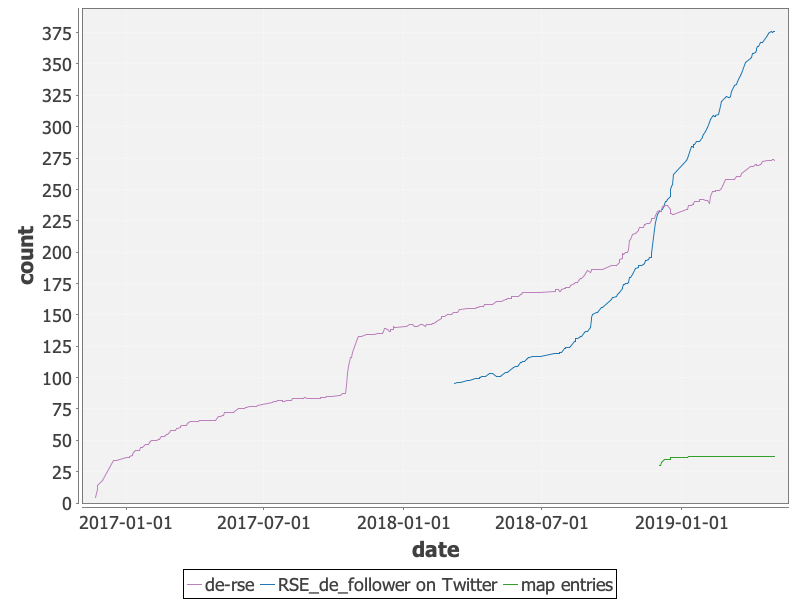
\includegraphics[width=.95\textwidth]{2019_05_mailinglist_counter}
  \caption{Abonnementenzahlen de-RSE Twitter, Mailingliste und Karte (Stand Mai 2019) \label{fig:abo201905}}
\end{figure}

\clearpage
\section{Tätigkeiten 2018 während der Vereinsexistenz}

\begin{itemize}
 \item \textbf{26.11.2018}\\
  Die \textbf{Gründungsversammlung} fand am 26. November 2018 beim Exzellenzcluster Bild Wissen Gestaltung -- Interdisziplinäres Labor der Humboldt-Universität zu Berlin in der Sophienstraße 22a, 10178 Berlin, statt.
  21 Personen nahmen teil und disktutierten die im Vorfeld erstellte Satzung und Geschäftsordnung, bevor schließlich der Verein gegründet und ein erster Vorstand gewählt wurde.
 \item \textbf{November \& Dezember 2018}\\
  Der Vorstand nahm die Arbeit auf und bereitet die Anmeldung im Vereinsregister vor.
  Bis zum Jahresende lag noch keine Informationen des zuständigen Amtsgerichts Charlottenburg vor, wodurch weitere notwendige Schritte (z.B. Vereinskonto, Beantragung der Gemeinnützigkeit) und die erste ordentliche Vorstandssitzung ins Jahr 2019 gelegt werden mussten.
\end{itemize}

%\section{Veranstaltungen}
%- deRSE-relevante Events, wo wir als Mitglieder auftraten
%- lokale RSE-Treffen, von deRSE-Mitgliedern organisiert

%\section{Lokale und regionale Gruppen}
%- Liste lokaler RSE-Gruppen evtl -> nur, wenn es nicht nur ein paar einzelne sind bisher

\end{document}
